\documentclass[blue]{beamer}
%\usetheme{Warsaw}
%\usetheme{Boadilla}
%\usetheme{CambridgeUS}
%\usetheme{Berlin}
%\usetheme{Frankfurt}
%\usetheme{Warsaw}
%\usetheme{AnnArbor}
%\usetheme{Antibes}
%\usetheme{Bergen}
%\usetheme{Berkeley}
%\usetheme{Berlin}
%\usetheme{Boadilla}
%\usetheme{boxes}
%\usetheme{CambridgeUS}
%\usetheme{Copenhagen}
%\usetheme{Darmstadt}
%\usetheme{default}
%\usetheme{Dresden}
%\usetheme{Frankfurt}
%\usetheme{Ilmenau}
%\usetheme{Goettingen}
%\usetheme{Hannover}
%\usetheme{JuanLesPins}
%\usetheme{Luebeck}
%\usetheme{Madrid}
%\usetheme{Malmoe}
\usepackage{graphicx}
%\usetheme{Marburg}
%\usetheme{Montpellier}
%\usetheme{PaloAlto}
%\usetheme{Pittsburgh}
%\usetheme{Rochester}
%\usetheme{Singapore}
%\usetheme{Szeged}
%\usepackage [autostyle, english = american]{csquotes}
%\MakeOuterQuote{"}
%\usecolortheme{dove}
%\usepackage{breqn}

\usepackage[english]{babel}
\usepackage[latin1]{inputenc}
\usepackage{bbm}
\setbeamercovered{transparent}

\title{Housing Investment during the Pandemic}
\subtitle{ }
\author[Karimzada, Khan and Yip]{Muhebulllah Karimzada, Shahed Khan and Terry Yip}
\institute{\textit{McMaster U., Western U. and McMaster U.}}
%\institute{Future of Growth Conference}
\bigskip
%\date[ ]{RCEA: 3rd Warsaw Money-Macro-Finance Conference (Online)}
\date[ ]{August 19, 2021}

\begin{document}
\frame{\titlepage}
\label{moti1}
\begin{frame} \frametitle{Motivation}
  We are trying to understand what explains the housing investment in Canada during the Pandemic 
 		 	\begin{itemize}	
 		 	    \item []
 		\item 	In March 2020, economic activities have been abruptly shut down and unemployment spiked as a consequence of lockdown orders \hfill \hyperlink{unemployment}{\beamergotobutton{Unempolyment rate}} 
 		   \item []
 		   \item According to the  Labour Force Survey, working from home increased from 4% to 32% during the Covid19 period
 		   \item []
 		\item  Governments increased public debt and used a broad set of  fiscal instruments to mitigate the crisis 
 		   \item []
 		   \item Bank of Canada used monetary policy to mitigate the crisis  \hfill \hyperlink{bank_rate}{\beamergotobutton{Bank rate}} 
 		   \item []
 		\item However the housing market recovered very quickly during the crisis \hfill \hyperlink{price}{\beamergotobutton{Home price rising}} 
          \end{itemize}
        
      %
\end{frame}



\begin{frame} \frametitle{Motivation}
\label{motivation}
 Suggested explanations: 
            \begin{itemize}    
                  \item Mortgage rates reduced significantly with the BoC's overnight rate cut to close to zero \\
                  \hfill \hyperlink{house_sales}{\beamergotobutton{Home sales}}  \hfill \hyperlink{mortgage}{\beamergotobutton{Mortgage payment}} \hfill \hyperlink{deferral}{\beamergotobutton{Mortgage deferrals}}
                  \item Government provided generous income support to households mostly affected by COVID-19 (such as CERB and other transfers)
                  \item In 2020 Q2, Canadians received more money from government aid programs than they lost in wages and salaries (\$56 billion vs \$23 billion). 
                  \item []
%             \linebreak
%         \item Explore if disappointment around the expected future path of financial reforms can shed light on the Korean sudden stop events of 1997-1999
%             \linebreak
%         \item Calibrate the model to the Korean economy in the 1990s to tease out quantitative implications. 
 \end{itemize}
 Other possible explanations: %Mechanism of this paper: 
  \begin{itemize}    
  \item The supply of homes tightens   \hfill \hyperlink{home_supply}{\beamergotobutton{Home supply tightens}}
  \item Working from homes is now reality for many Canadians
       \hfill \hyperlink{moving_out}{\beamergotobutton{Moving out}}  
  
   \end{itemize}
      %
\end{frame}




\begin{frame} \frametitle{Outline of the model}

The model environment closely follows Iacoveillo and Neri (2010).
\begin{itemize}
\item Two types of households: patient and impatient
\item []
\item Both types of HHs consume, work in two sectors (consumption sectors and housing sectors), and accumulate housing
\item []
\item HHs can work at office or from home for consumption good sectors
\item []
\item Unlike patient HHs, impatient HHs don't own capital or firms. Their borrowing limits are constrained by a fraction of the expected present value of their next period's housing stock.
\item []
\item Other agents:  firms,  retailers and monetary policy authority
              \end{itemize}
          \end{frame}
         

\begin{frame} \frametitle{Patient Households}
\small
\begin{itemize}
\item The representative patient household maximizes  life-time utility function of the form 
\[
		E_0 \sum_{t=0}^{\infty} \beta^t  \left(ln(c_t-\epsilon c_{t-1}) + j_t \ln h_t - \frac{\tau_t}{1+\eta} (n_{o,t}^{1+\xi}+ n_{wh,t}^{1+\xi}  + n_{h,t}^{1+\xi} ) ^{\frac{1+\eta}{1+\xi}} \right)
\]
where, 
${n_{c,t} = n_{o,t} + \chi n_{wh,t}^{\alpha_o} h_t^{1-\alpha_o} } $

%\[
%	{n_{c,t} = \left( \omega_o n_{o,t}^{1+\xi_n} + (1-\omega_o)  ( n_{wh,t}^{\alpha_o} h_t^{1-\alpha_o}  )^{1+\xi_n}\right)^{\frac{1}{1+\xi_n}}  }
%\]
\item []
\item The budget constraint is
\begin{multline} \label{eq:patient_hh_BC}
	c_t + \frac{k_{c,t}}{A_{k,t}} + k_{h,t}  + q_t h_t + s_t = w_{c,t}n_{c,t} + w_{h,t}n_{h,t}+(R_{c,t}  + \frac{1-\delta_{kc}}{A_{k,t}})k_{c,t-1}\\ +  \left(R_{h,t}+1-\delta_{kh}\right)k_{h,t-1} + \frac{R_{t-1}s_{t-1}}{\pi_t} 
		 + q_t (1-\delta_h) h_{t-1} 
	\end{multline}
\end{itemize}
\end{frame}


\begin{frame} \frametitle{Impatient Households}
\small
\begin{itemize}
\item The impatient household maximizes the following:
\[
E_0 \sum_{t=0}^{\infty} \beta'^t  \left(\ln(c'_t - \epsilon' c'_{t-1}) + j_t \ln h_t' - \frac{\tau_t}{1+\eta'}  (n_{o,t}^{'1+\xi}+ n_{wh,t}^{'1+\xi}  + n_{h,t}^{'1+\xi} ) ^{\frac{1+\eta'}{1+\xi}}  \right)
\]
where, 
${n_{c,t}' = n_{o,t}' + \chi n_{wh,t}^{'\alpha_o} h_t^{'1-\alpha_o} }$
\item []
\item The budget constraint is 
	\begin{equation}\label{eq:impatient_hh_BC}
		c'_t + q_t h'_t + \frac{R_{t-1}b_{t-1}}{\pi_t}  = w'_{c,t}n'_{c,t} + w'_{h,t}n'_{h,t}  + q_t (1-\delta_h) h'_{t-1} + b_t   
	\end{equation} 
	\item The borrowing constraint is 
	\begin{equation}\label{eq:BC}
		b_t \leq m E_t\left(\frac{q_{t+1}h'_t \pi_{t+1}}{R_t}\right)
	\end{equation}
	\end{itemize}
	\end{frame}
	
	\begin{frame}\frametitle{Technology and Firms}
	\small
	\begin{itemize}
\item The  firm hires labour and capital  to produce wholesale goods $Y_t$ and new houses $IH_t$. It maximizes the following:
\begin{multline} 
	\	\max \frac{Y_t}{X_t} + q_t IH_t - \big[\sum_{i=c,h} w_{i,t} n_{i,t} + \sum_{i=c,h} w'_{i,t}n'_{i,t} + \sum_{i=c,h} R_{i,t}  k_{i,t-1} 
	 \big]
\end{multline} 
%where $X_t$ is the markup of final goods over wholesale goods.
	\item The production technologies are:
	\begin{equation}
		Y_t = \left(A_{c,t}(n_{c,t}^\alpha n_{c,t}^{'1-\alpha})\right)^{1-\mu_c} (k_{c,t-1})^{\mu_c}
	\end{equation}
	\begin{equation}
		IH_t = \left(A_{h,t} (n_{h,t}^\alpha n_{h,t}^{'1-\alpha})\right)^{1-\mu_h} (k_{h,t-1})^{\mu_h} 
	\end{equation}
\end{itemize}
	\end{frame}
	
\begin{frame}
\frametitle{Data and estimation}
\label{main}      
 \begin{itemize}
 \item The model is estimated for Canada using Bayesian estimation technique
\item []
 \item 11 observables: consumption, inflation, housing investment, capital investment, labor hours in consumption sector, labor hours in housing sector, house price index, bank rate, wages in consumption sector, wages in housing sector and GDP
\item []
 \item Time periods: 1997:Q1 to 2021:Q1
\item []
\item 7 shocks: Prod. consumption sector, prod. housing sector, prod. capital sector, housing preference, labor supply, cost push and monetary policy
 \end{itemize}
 \end{frame}
 
 
 
 
 \begin{frame}
 	\frametitle{Data and estimation}
 	We choose parameters ($\beta$, $\chi,$ $j$, $m$, and $\mu_c$) to target the following data moment:
 	\begin{table}[htbp]
 		\centering
 		\caption{Data Moments}
 		\begin{tabular}{lr} 
 			\hline
 			Housing Investment to GDP & 6\% \\
 			Investment to GDP & 11\% \\
 			Working from Home Ratio & 4\% \\
 			Loan to Value Ratio & 60\% \\
 			Annual interest Rate  & 3\% \\
 			\hline
 		\end{tabular}%
 		\label{tab:addlabel}%
 	\end{table}%
 \end{frame}
 
 
 
 
 
 
 
 
 
 
 
 
 
 
 
\begin{frame}
\frametitle{\small{Variance decomposition }}
\begin{table}[htbp]
\setlength{\belowcaptionskip}{4pt}
%\renewcommand{\baselinestretch}{1.35}\small\normalsize
\begin{center}
%\caption{\footnotesize Variance Decomposition Based on the Estimated Parameter Values}
\scalebox{0.59}{
\begin{tabular*}{1.7\textwidth}%
{@{\extracolsep{\fill}}ccccccccc} \hline\hline
\multicolumn{1}{l}{\footnotesize \textbf{Observables}} & \footnotesize
\textbf{$C-Tech$} & \footnotesize \textbf{$IH-Tech$} &
\footnotesize \textbf{\textit{$IK-Tech$} }&
\footnotesize {\textit{H-Pref.} }&
\footnotesize {\textit{Monetary pol.} }&
\footnotesize {\textit{L supply} }&
\footnotesize {\textit{Cost push} }&
\footnotesize {\textit{ME} }
\\ \hline
\\
C&31.76&0.03&2.88&0.72&43.65&3.83&17.13&0\\
$\pi$&3.99&0.1&16.92&0.08&9.63&1.59&67.69&0\\
$I_{H}$&0.01&85.14&0.11&1.78&0.01&12.95&0&0\\
$I_{K}$&0.24&0&55.12&0&6.78&0.09&1.96&35.8\\
$N_{C}$&0.51&0.02&58.37&0.14&0.77&39.94&0.24&0\\
$N_{H}$&0&34.54&0.47&7.86&0.02&57.1&0&0\\
$Q$&12.44&0.46&1.25&12.06&56.18&0.89&16.71&0\\
$R$&8.84&0.25&25.44&0.07&46.72&2.25&16.44&0\\
$W_{C}$&3.96&0&16.85&0.07&21.28&10.01&6.76&41.08\\
$W_{H}$&5.52&16.4&0.36&2.15&24.2&4.3&7.32&39.74\\
GDP&26.89&0.84&24.05&0.35&1&21.53&0.3&25.05\\
\hline
\end{tabular*}}
 \label{VD Covid}
\end{center}
\end{table}
 
\end{frame} 
 
 
\begin{frame}
  \frametitle{IRFs to Productivity Shock}
\begin{figure}
    \begin{center}
      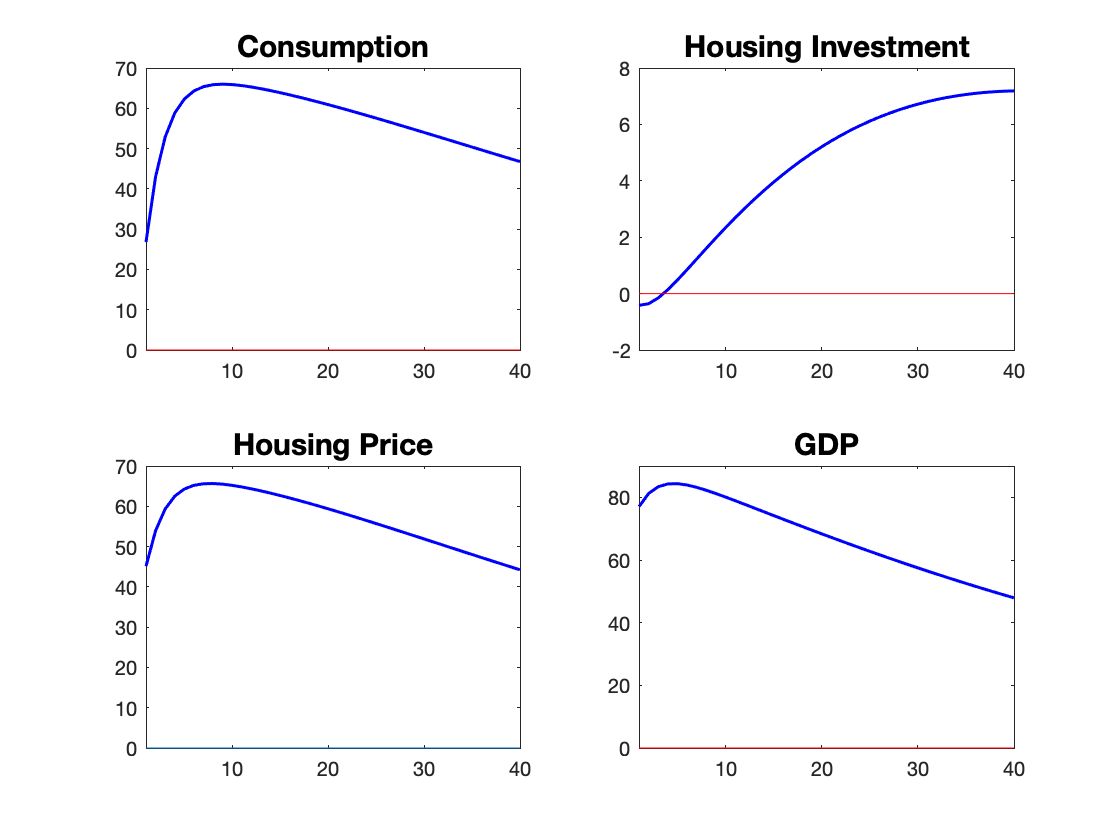
\includegraphics[scale=0.27]{C_shock.png}
      %    \includegraphics[scale=.40]{one.pdf}
      \end{center}
  \end{figure}
\end{frame}

\begin{frame}
  \frametitle{IRFs to Monetary Shock}
\begin{figure}
    \begin{center}
      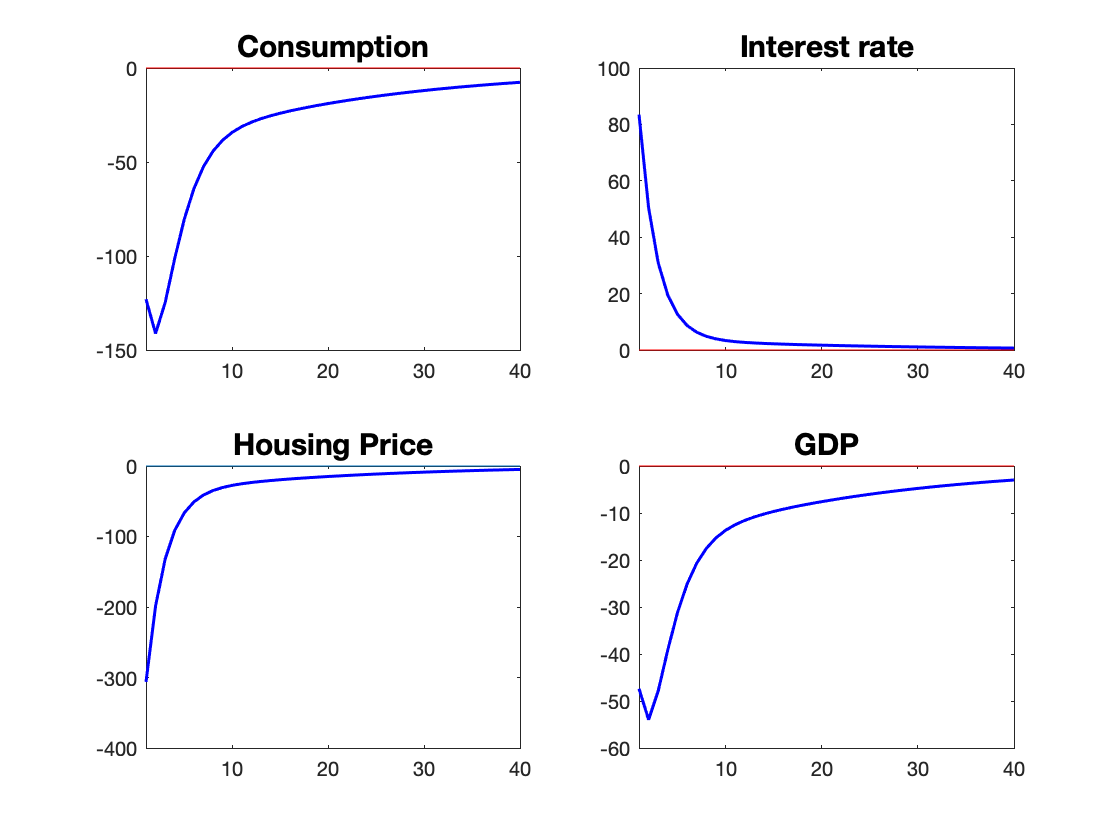
\includegraphics[scale=0.27]{monetary_shock.png}
      %    \includegraphics[scale=.40]{one.pdf}
      \end{center}
  \end{figure}
\end{frame}

\begin{frame}
  \frametitle{IRFs to working from home shock}
\begin{figure}
    \begin{center}
      
\includegraphics[scale=0.27]{wfh_shock.png}
      %    \includegraphics[scale=.40]{one.pdf}
      \end{center}
  \end{figure}
\end{frame}



%\begin{frame}
%\frametitle{Historical and smoothed variables}
%\begin{figure}
 %   \begin{center}
   %  \includegraphics[scale=.41]{jk1.pdf}
     % \includegraphics[scale=.61]{shock_default.png}
  %    \end{center}
  %\end{figure}
%\end{frame}






\begin{frame}
  \frametitle{Simulated House Prices (Level) with 3 Different Scenarios  }
\begin{figure}
    \begin{center}
      
\includegraphics[scale=0.45]{Q_level_simu_vs_data.pdf}
      %    \includegraphics[scale=.40]{one.pdf}
      \end{center}
  \end{figure}
\end{frame}


\begin{frame}
  \frametitle{Simulated House Prices (Growth) with 3 Different Scenarios ( }
\begin{figure}
    \begin{center}
      
\includegraphics[scale=0.45]{Q_growth_simu_vs_data.pdf}
      %    \includegraphics[scale=.40]{one.pdf}
      \end{center}
  \end{figure}
\end{frame}







\begin{frame}
  \frametitle{Conclusions}
\begin{itemize}
\item  We introduced working from home to the Iacoveillo and Neri (2010) model and estimated it for Canada using Bayesian estimation technique
\item []
\item Our preliminary results show that monetary policy shocks and supply shocks are more important than demand shocks to explain the home price movement during the Pandemic
\item []
%\item Interm. cost shocks can explain the boom and burst episode. 
\item Future plan: adding government sector to the model to capture the effects of fiscal policy during the Pandemic
\item []
  \end{itemize}
\end{frame}


\begin{frame}
  \frametitle{Home resales rebound quickly}
  \label{house_sales}
\begin{figure}
    \begin{center}
     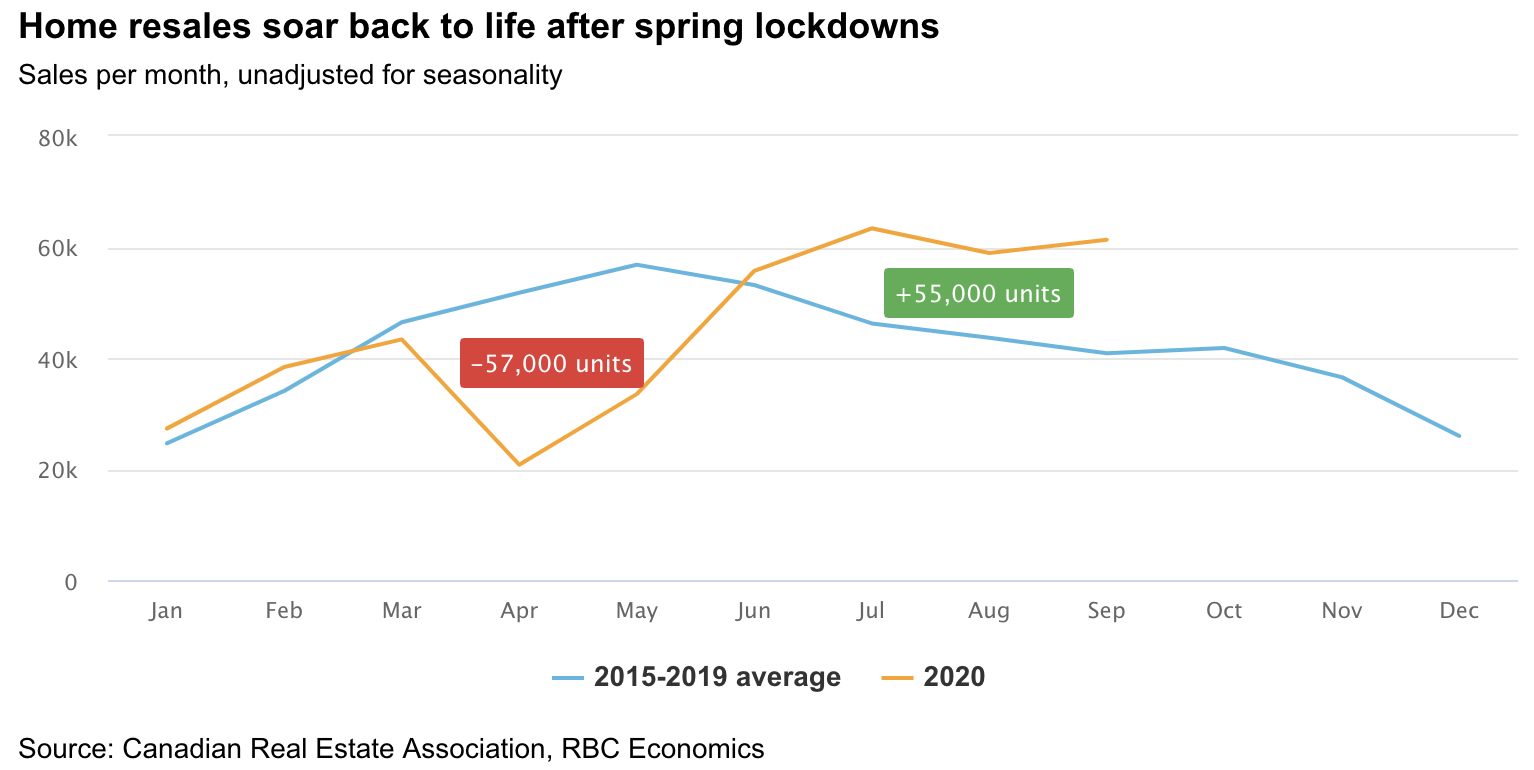
\includegraphics[scale=.43]{KKT1.png}
      \end{center}
  \end{figure}
   \hfill \hyperlink{motivation}{\beamergotobutton{back}}
\end{frame}

\begin{frame}
  \frametitle{Monthly mortgage payment declines}
    \label{mortgage}
\begin{figure}
    \begin{center}
     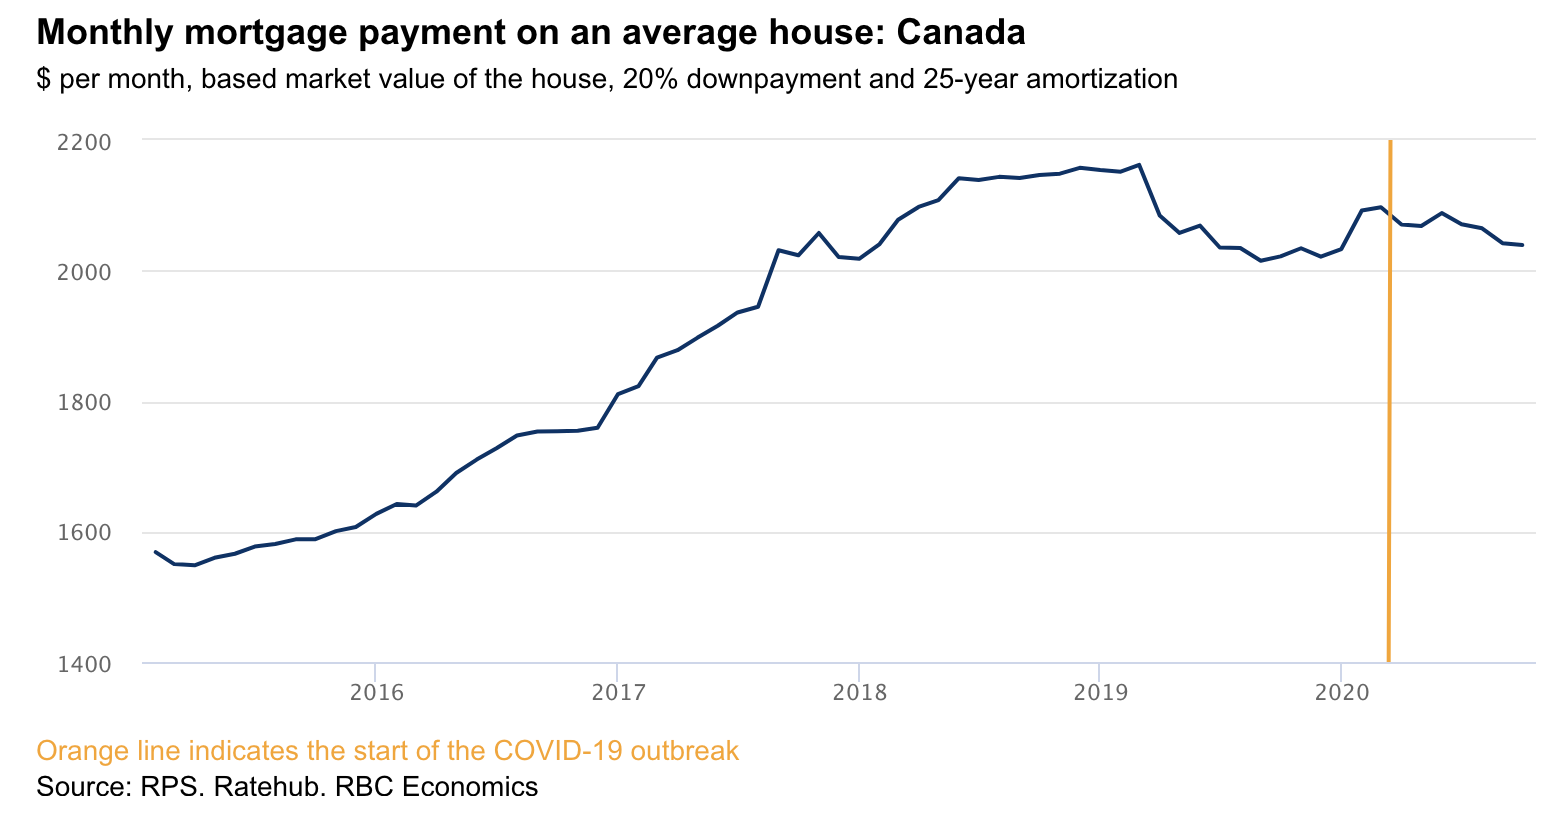
\includegraphics[scale=.42]{KKT2.png}
      \end{center}
  \end{figure}
    \hfill \hyperlink{motivation}{\beamergotobutton{back}}
\end{frame}

\begin{frame}
  \frametitle{Mortgage payment deferrals}
     \label{deferral}
\begin{figure}
    \begin{center}
     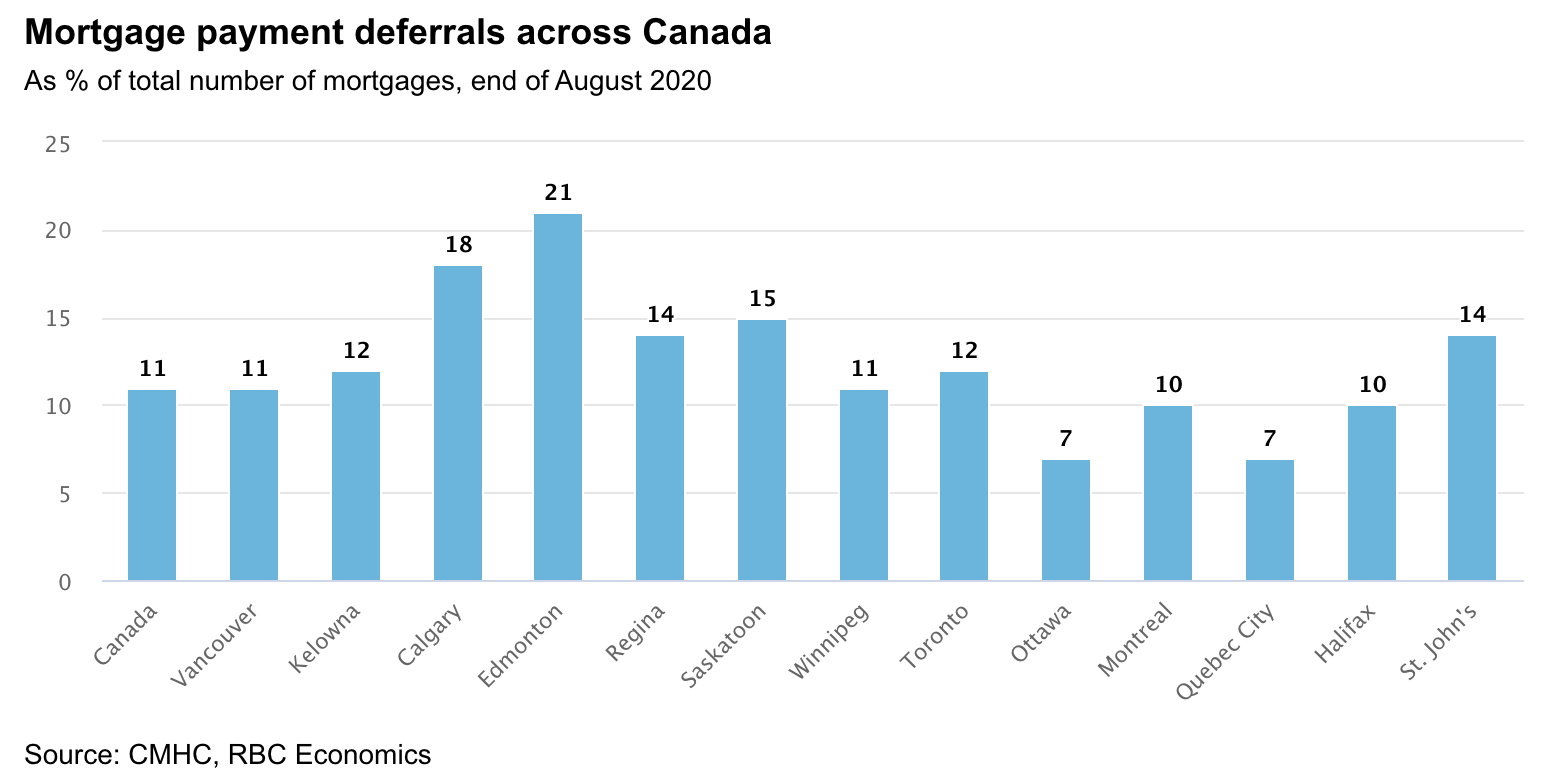
\includegraphics[scale=.41]{KKT3.png}
      \end{center}
  \end{figure}
  \hfill \hyperlink{motivation}{\beamergotobutton{back}}
\end{frame}

\begin{frame}
  \frametitle{Home supply tightens}
  \label{home_supply}
\begin{figure}
    \begin{center}
     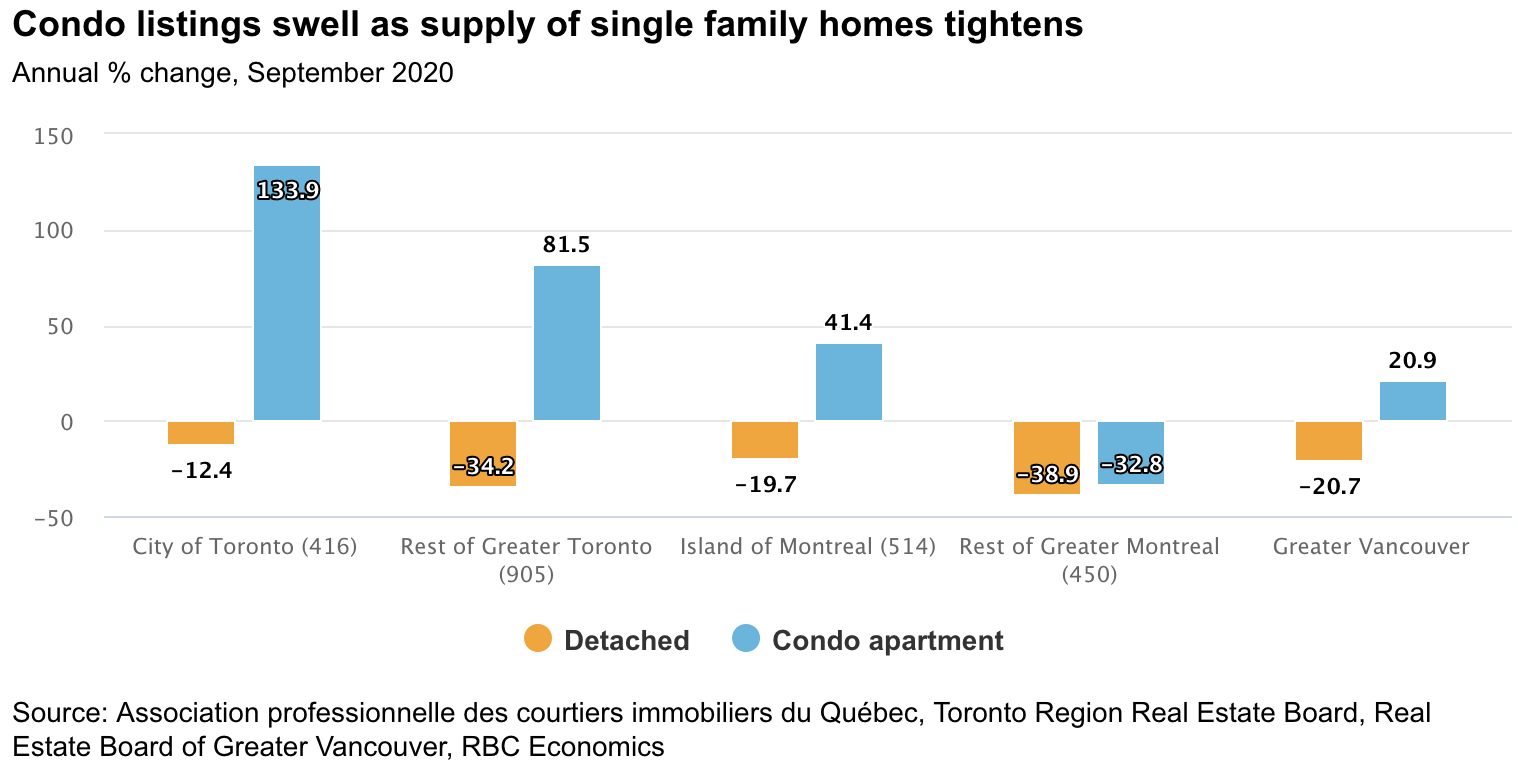
\includegraphics[scale=.43]{KKT4.png}
      \end{center}
  \end{figure}
    \hfill \hyperlink{motivation}{\beamergotobutton{back}}
\end{frame}

\begin{frame}
  \frametitle{Moving out of big cities}
  \label{moving_out}
\begin{figure}
    \begin{center}
     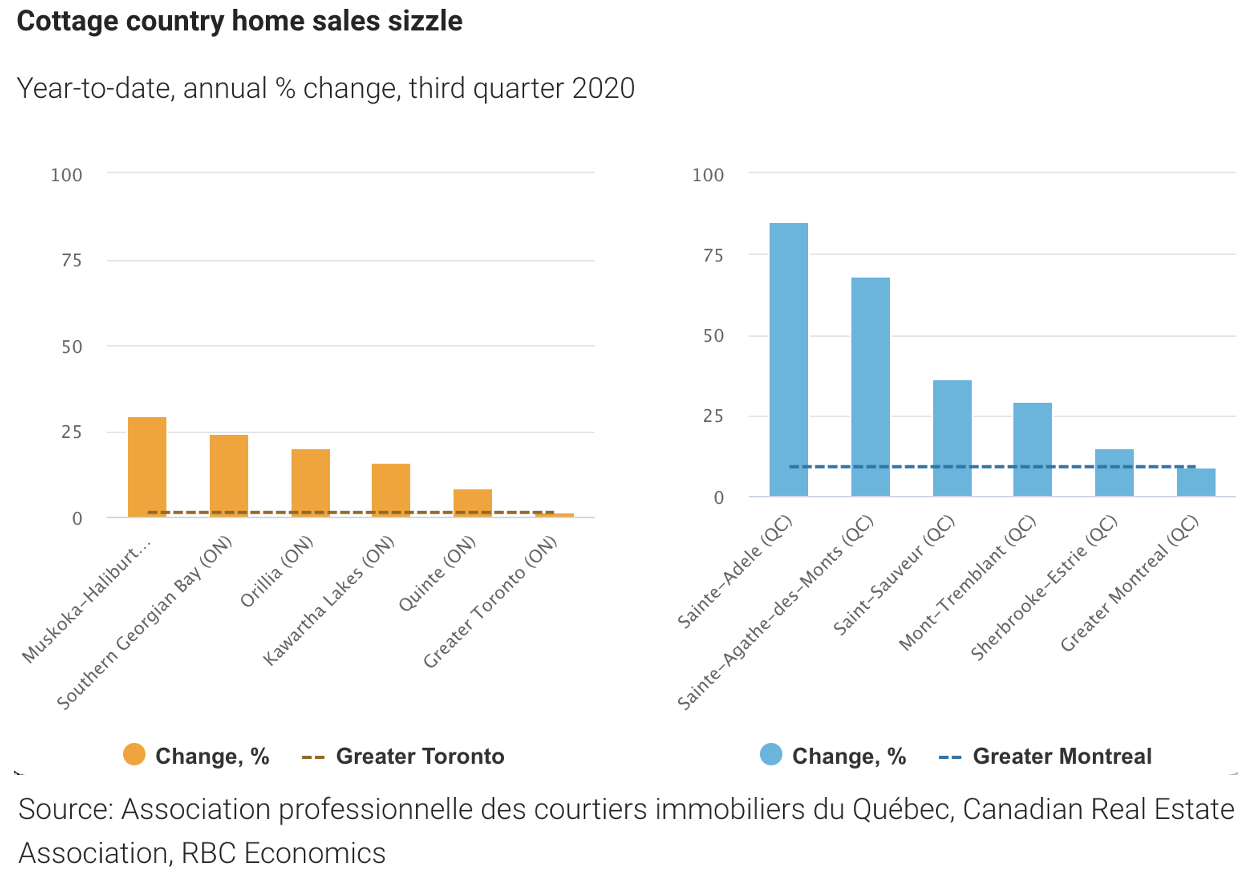
\includegraphics[scale=.47]{KKT5a.png}
      \end{center}
  \end{figure}
    \hfill \hyperlink{motivation}{\beamergotobutton{back}}
\end{frame}

\begin{frame}
  \frametitle{Home price increasing}
  \label{price}
\begin{figure}
    \begin{center}
     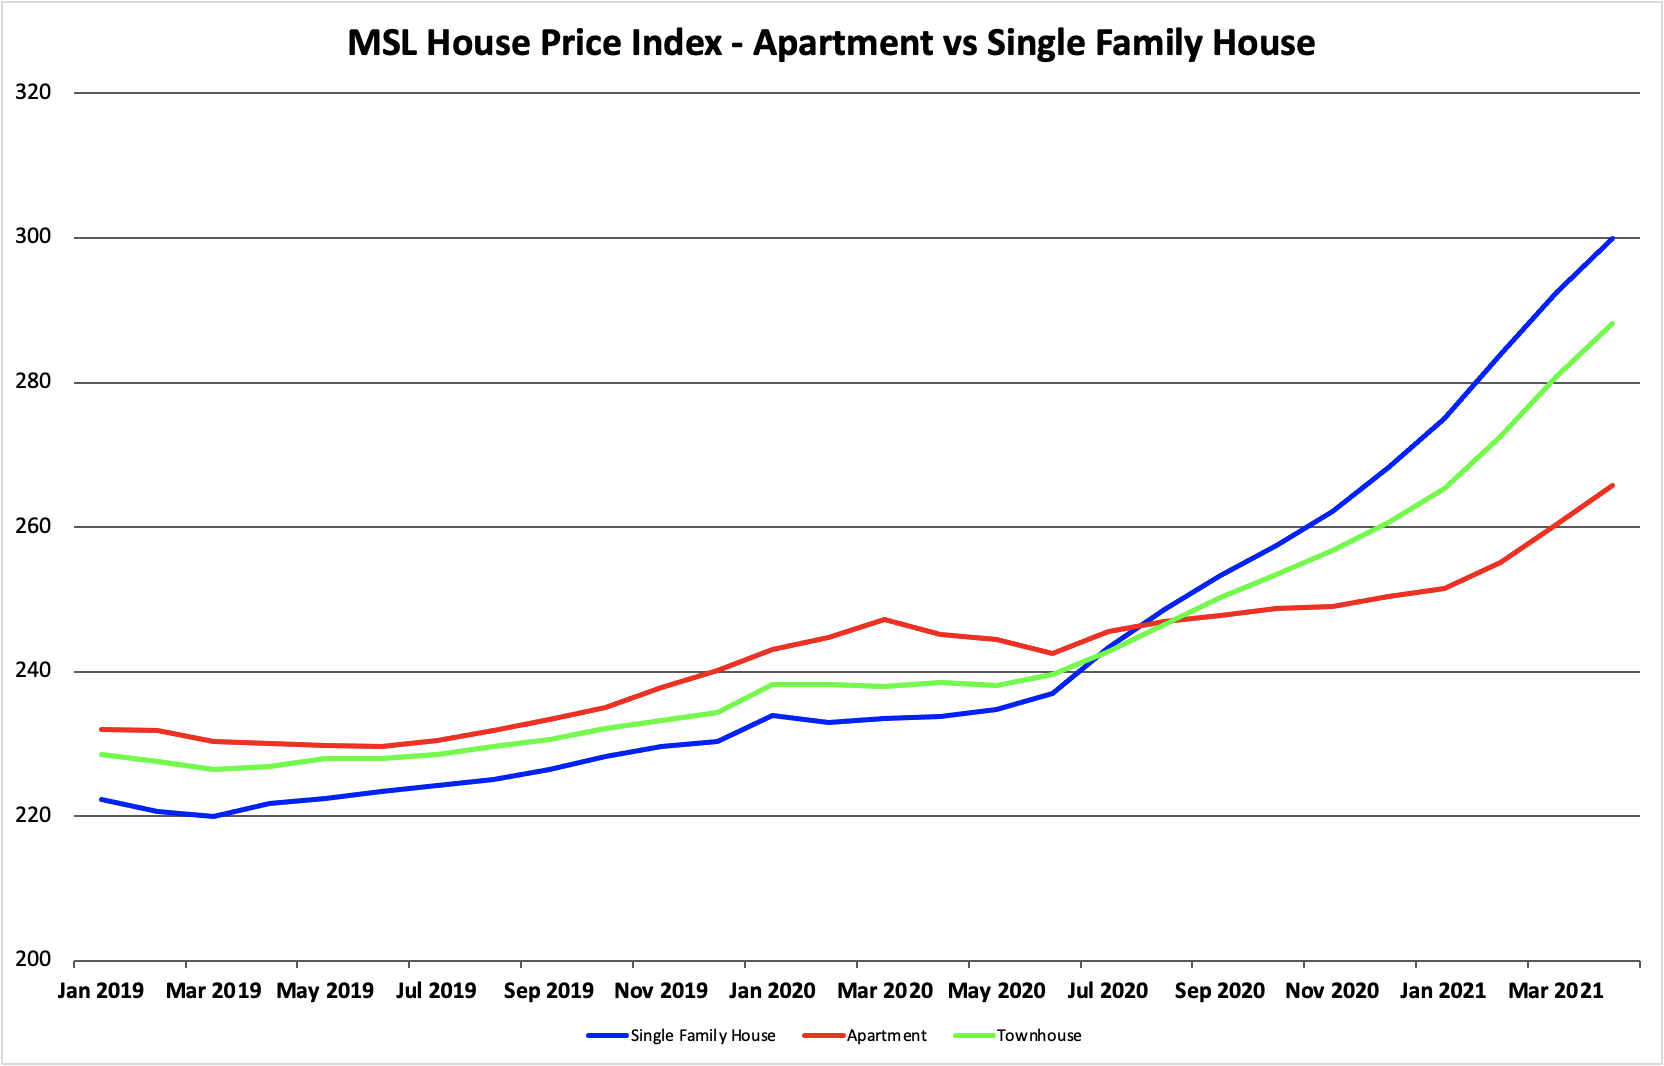
\includegraphics[scale=.17]{KKT6a.png}
      \end{center}
  \end{figure}
    \hfill \hyperlink{moti1}{\beamergotobutton{back}}
\end{frame}




\begin{frame}
  \frametitle{Unemployment rate}
  \label{unemployment}
\begin{figure}
    \begin{center}
     
\includegraphics[scale=.30]{unemployment.png}
      \end{center}
  \end{figure}
   \hfill \hyperlink{moti1}{\beamergotobutton{back}}
\end{frame}


\begin{frame}
  \frametitle{Overnight loan rate}
  \label{bank_rate}
\begin{figure}
    \begin{center}
     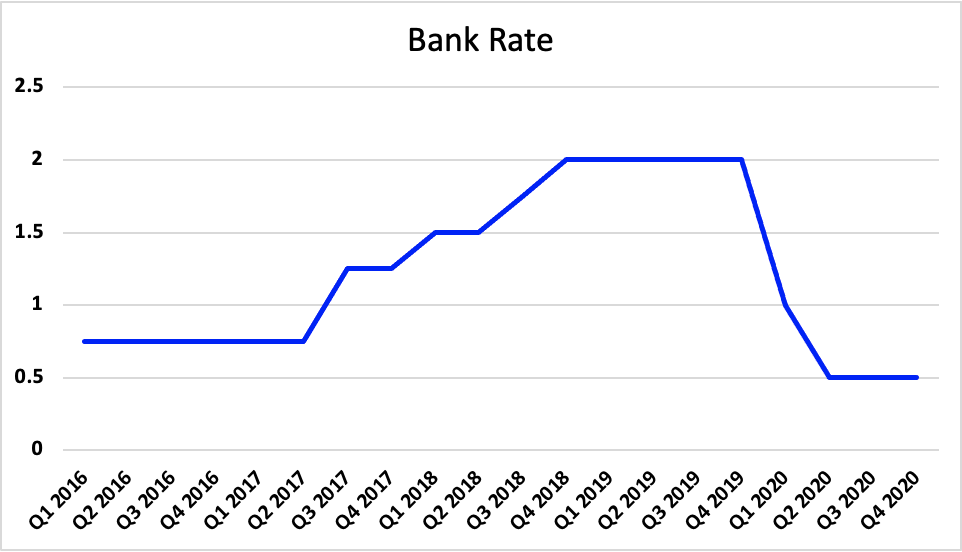
\includegraphics[scale=.32]{bank_rate.png}
      \end{center}
  \end{figure}
   \hfill \hyperlink{moti1}{\beamergotobutton{back}}
\end{frame}







\end{document}
